\documentclass{article}

% if you need to pass options to natbib, use, e.g.:
\PassOptionsToPackage{numbers}{natbib}
% before loading nips_2017
%
% to avoid loading the natbib package, add option nonatbib:
% \usepackage[nonatbib]{nips_2017}

%\usepackage{nips_2017}

% to compile a camera-ready version, add the [final] option, e.g.:
\usepackage[final]{nips_2018}

\usepackage[utf8]{inputenc} % allow utf-8 input
\usepackage[T1]{fontenc}    % use 8-bit T1 fonts
\usepackage{hyperref}       % hyperlinks
\usepackage{url}            % simple URL typesetting
\usepackage{booktabs}       % professional-quality tables
\usepackage{amsfonts}       % blackboard math symbols
\usepackage{nicefrac}       % compact symbols for 1/2, etc.
\usepackage{microtype}      % microtypography
\usepackage{graphicx}
\usepackage{amsmath}

\bibliographystyle{plainnat}

\title{Predicting Future Events in a Complex Time Series Using an Adaptive Deep LSTM Ensemble}

% The \author macro works with any number of authors. There are two
% commands used to separate the names and addresses of multiple
% authors: \And and \AND.
%
% Using \And between authors leaves it to LaTeX to determine where to
% break the lines. Using \AND forces a line break at that point. So,
% if LaTeX puts 3 of 4 authors names on the first line, and the last
% on the second line, try using \AND instead of \And before the third
% author name.

\author{Anthony Morast\\
		South Dakota School of Mines and Technology\\
        anthony.morast@mines.sdsmt.edu}

\begin{document}

\maketitle

\begin{abstract}
  Deep learning methods are typically based on the assumption that a dataset's underlying data generating process does not change over time. However, for many important datasets these assumptions don't hold resulting in non-stationarity. Learning algorithms operating in non-stationary settings often produce unreliable and spurious results leading to poor understanding and forecasting. Two common remedies to this ailment are to i) train a combination of methods and perform online model selection and ii) retrain a model repeatedly throughout time. In this paper an Adaptive Deep LSTM Ensemble (ADLE) is introduced that takes advantage of both of the aforementioned methodologies. It is shown that ADLE performs competitively with state-of-the-art LSTM and ARIMA models. 
\end{abstract}

\section{Introduction}

Since its inception, deep learning has proved wildly successful on many classification and regression tasks. However, deep learning methods are typically based on the assumption that the underlying data generating process does not change over time. This property is known as stationarity and, in many sufficiently complex time series, the assumption does not hold. Using non-stationary data in time series models often produces unreliable and spurious results and leads to poor understanding and forecasting.

Non-stationary time series data is characterized by changing statistical properties in its data generating function. Put another way, through time, the data making up the time series will be drawn from distributions parameterized by different statistics, e.g. normal distributions parameterized by different means ($\mu$) and variances ($\sigma^2$). Machine learning algorithms typically have no mechanism to account for this change in statistical properties making learning in non-stationary environments difficult.

Two possibilities for effectively handling non-stationary data are to use a combination of different models and perform online model selection and to retrain a model repeatedly on either a finite window into the past or on all available data. When implementing state-of-the art models for non-stationary time series, such as the ARIMA model, one usually takes advantage of the latter. The proposed adaptive ensemble combines both of these strategies into a model for one-step ahead predictions of non-stationary time series data.

This work introduces an adaptive ensemble of deep (stacked) LSTM-RNNs to model a non-stationary time series. The ensemble trains a set of LSTM networks on different subsets of the available training data to be used for forecasting. The outputs of the networks are combined by a function taking into consideration the statistical properties of the data segment used to train a network and the current statistical properties of a sliding window over the data. As new data become available additional networks are added to the ensemble increasing its effectiveness over time and allowing the ensemble to adapt. It's shown that this strategy yields competitive results when compared to ARIMA models and single LSTMs.


\section{Related Work}

One particularly challenging aspect of learning in non-stationary environments is that changes in non-stationary time series may be abrupt or gradual, random or systematic, and may even be cyclical. Much work has been done to handle these particular difficulties and typically include mechanisms to detect the changes, learn the changes, or forget past trends in the time series. Ensemble algorithms, in particular, typically try to update the weighting mechanisms of a fixed set of methods, use new data to update an ensemble of methods, and/or add new methods to the ensemble as training data become available. A review of strategies for building ensembles to operate in non-stationary environments is provided by Kuncheva \citep{kuncheva2004classifier}.

In the past different variations of ensemble methods have been applied to learning non-stationary time series data, many of which focus on classification rather than regression. Heeswijk \citep{van2009adaptive} uses an ensemble of extreme learning machines (ELMs) for prediction in both stationary and non-stationary environments. The ensemble adapts by adjusting the weights of the ensemble's aggregation methodology. In this ensemble, the non-stationarity is dealt with by creating the ELMs with various hyperparameters making in an attempt to find the hyperparameters that work best in the current environment. A major drawback of this ensemble is the need to retrain at each time step. 

Polikar \citep{muhlbaier2007ensemble} introduces an ensemble for classification in non-stationary environments. The ensemble adds new classifiers as training data become available and, like Heeswijk \citep{van2009adaptive}, uses a weighting scheme based on each classifier's current performance. Blum \citep{blum1995empirical} proposes an ensemble method focusing on different weighting schemes for the ensemble. Yet another approach at adaptation is the removal of ensemble methods once a change is detected (Chu \citep{chu2004fast}) or on other heuristics (Street \citep{street2001streaming}), keeping the ensemble a fixed size. Other ensembles rely heavily on training data for the preprocessing required to create the ensemble (Yu \citep{yu2008forecasting}) and combine aggregation methods to create a better classification methodology (Kotsiantis \citep{kotsiantis2010combinational}).

The proposed method takes advantage of two of the three mechanisms typically used to deal with non-stationary data. An ensemble is created which uses a dynamic weighting mechanism based on certain statistical properties of the data. Then, as new data become available, new methods will be added to the ensemble to more accurately represent the changes in the data. The proposed method does not retrain any of its members with newly acquired data which, after initial training, makes use of the algorithm more efficient. 


\section{Method}

\begin{figure}
\centering
\minipage{0.49\textwidth}
	\centering
  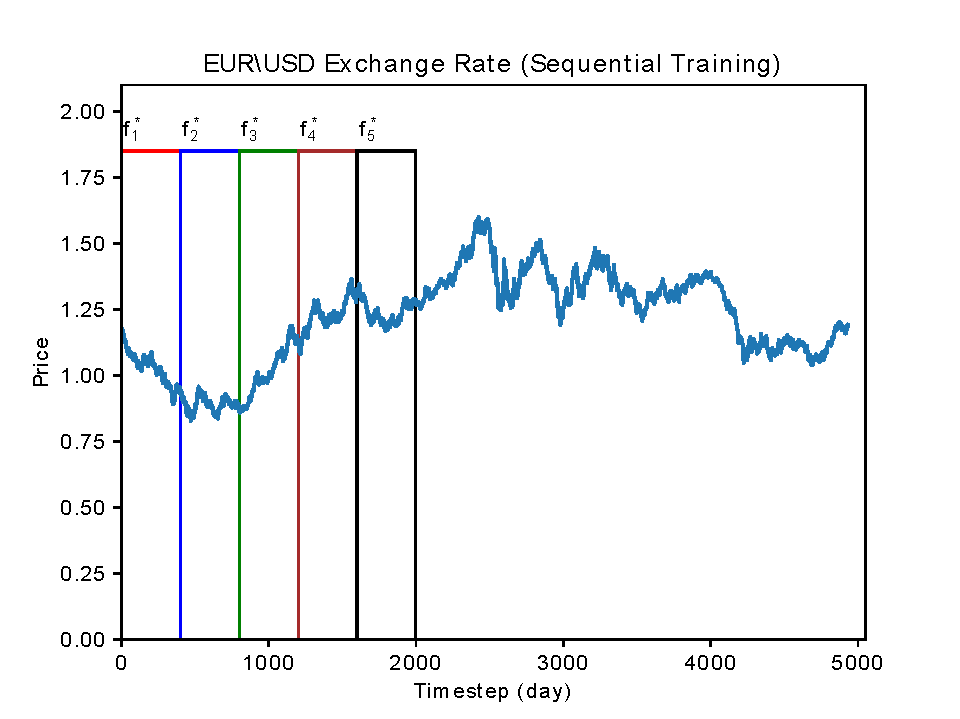
\includegraphics[scale=0.31]{imgs/sequential_forex.pdf}
  \caption{Segments of the training data when training the ensemble on sequential segments.}\label{fig:sequential}
\endminipage\hfill
\minipage{0.49\textwidth}
	\centering
  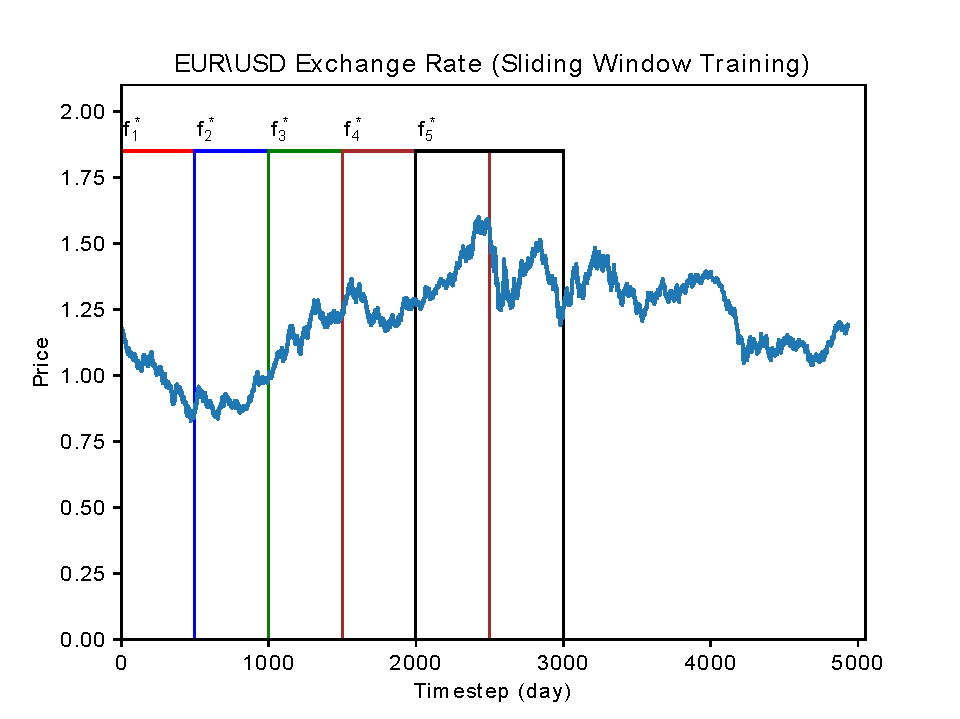
\includegraphics[scale=0.31]{imgs/overlap_forex.pdf}
  \caption{Segmentation of the training data with overlap on the various segments.}\label{fig:overlap}
\endminipage\hfill
% \minipage{0.32\textwidth}
%   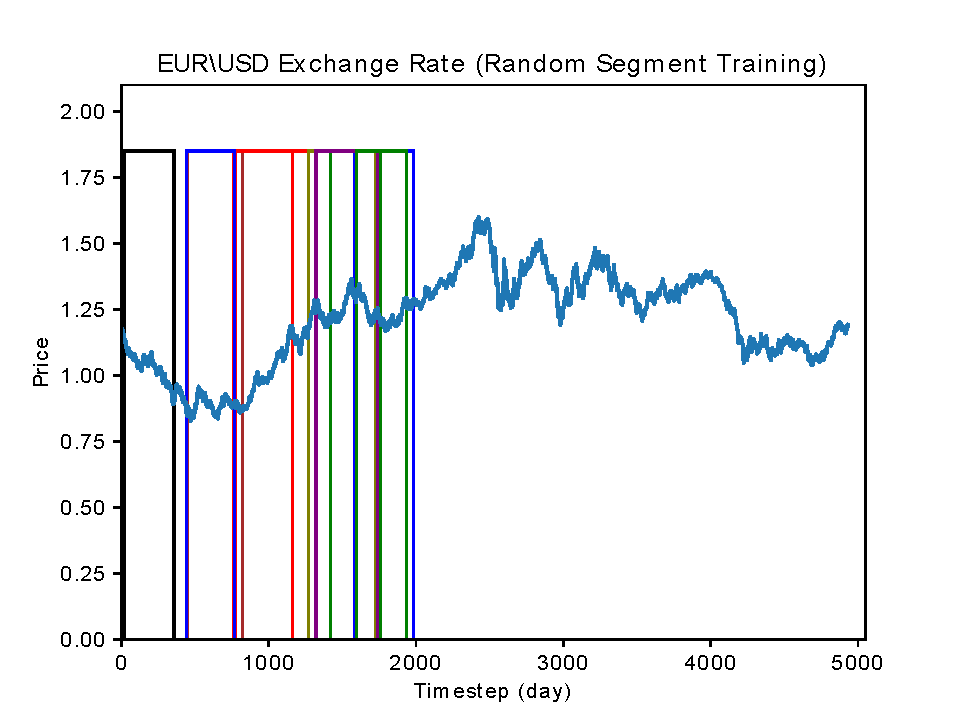
\includegraphics[scale=0.31]{imgs/random_segments_forex.pdf}
%   \caption{Training segments when start points and sizes are randomly generated.}\label{fig:random}
% \endminipage
\end{figure}

In traditional neural networks it is assumed that inputs are independent of one another. \textbf{Recurrent neural networks} (RNNs) remove this restriction by allowing current computations to be dependent on input, output, or hidden layer computations from previous time steps, making them ideal for modeling sequential data. Because of this dependency, RNNs are particularly susceptible to problems with vanishing and exploding gradients as errors are back-propagated through time. The accepted solution to these gradient problems in RNNs is to build the network with \textbf{long short-term memory} (LSTM) cells which use input, output, and forget gates to determine which data is relevant to the network and cell state \citep{hochreiter1997long}.

Because learning algorithms operating in non-stationary environments rely on up-to-date data, the model requires the ability to change with the environment, i.e. to adapt. This is usually done by retraining the model(s) as new data become available. This approach to adaptive learning is called \textbf{passive adaption} and typically requires frequently performing the lengthy training process consuming time and resources.

Ensemble methods improve machine learning results by aggregating the predictions of several base models which offers improved generalization and robustness over a single estimator. A particular kind of ensemble learning called \textbf{stacking} combines the predictions of several models trained on the available data with a combiner method, such as k-nearest neighbors or a neural network. Stacking ensemble methods have been successfully applied to many supervised and unsupervised machine learning tasks.

The proposed adaptive deep LSTM ensemble (ADLE), combines the prediction of an ensemble of LSTM recurrent neural networks. The networks are trained using one of two methodologies: i) sliding window wherein the network's training data is taken from a sliding window over the training data set and ii) sequential where the training data is broken into $s$ segments of equal size and uses one segment per network. These methodologies are depicted in Figures \ref{fig:sequential} and \ref{fig:overlap}. %, and \ref{fig:random}. , and iii) random segments where each network's training data is a randomly sized and selected segment of the training data

The aggregation of the predictions is done via a distance weighted $k$-NN algorithm. Weights are assigned to each network's prediction based on the distance the network's statistical properties are from the current statistical properties of a sliding window over the dataset. The $i^{th}$ network's weight is determined as
$$
	w_i = \frac{1}{d(x_q, x_i)^2}
$$
where $d(x_q, x_i)$ is the distance function defined as $d(x_q, x_i) = \sqrt{(\mu_q - \mu_i)^2 + (\sigma^2_q - \sigma^2_i)^2}$ where $\sigma^2_q \textnormal{ and } \mu_q$ are the variance and mean of the sliding window and $\sigma^2_i \textnormal{ and } \mu_i$ are the variance and mean of the $i^{th}$ network. Then the final prediction is, 
$$
	\hat{y} = \frac{\sum_{i=1}^k w_i\hat{y}_i}{\sum_{i=1}^k w_i}
$$
where $\hat{y}_i$ is the prediction from the $i^{th}$ network and $k$ is the number of neighbors being considered. In this prototypical implementation of ADLE, $k$ is equal to the number of networks in the ensemble. That is, each network's prediction is considered in the final prediction. Further work would include trying different values of $k$.

To adapt in changing non-stationary environments ADLE continuously adds new models to the ensemble as training data become available. As predictions are made with the ensemble, the time series values $x_t$ and their target values $y_t$ are stored in a list of historical points. As soon as the list contains enough feature/target pairs, $\{x_t, y_t\}$, to train a new LSTM network  an LSTM is trained and added to the ensemble. This procedure provides the ensemble functional approximations of the most recent data as well as additional robustness as the new data segments may have statistical properties not yet seen by the ensemble's other networks. 

Note that, in practice, training new ensembles will have little effect on the use of time and computational resources since data will become available gradually. Consider using the ensemble for one-step-ahead predictions on daily foreign exchange rate data. Then, if each ensemble method is trained on $500$ examples, it would take $501$ days until the list of historical points contains enough data to train a new network ($501$ rather than $500$ since $y_t = x_{t+1}$). This means training a new ensemble would be rare and not take too heavy a toll on computational resources.

Essentially, ADLE attempts to approximate different functions, $f^*_i$, using different segments of the training data to try and capture the changes in statistical properties of the time series data. Each method is added to a `dictionary' tying the statistical properties of the training segments to a network trained to approximate that segment, $\{\sigma_i, \mu_i : f^*_i\}$. The dictionary is then queried for predictions from networks trained over data with similar statistical structures as a sliding window over the most recent data. Each selected network's prediction is then weighted based on this distance.

The key benefits of ADLE over other ensemble methods are the train-once mentality, weights being determined instantaneously rather than being trained over time, and the use of strong learners \textit{viz.} LSTM-RNNs. Many ensemble methods require constant retraining, some prior to every prediction, which uses time and computational resources. The networks in ADLE are trained once on their segment of the data and the ensemble adapts by adding new methods to the ensemble. Considering the statistical properties of the time series as a weighting mechanism allows changes, gradual or abrupt, to be determined as quickly as they occur and, unlike many other ensembles, the methods that  ADLE consists of are well-suited to learn very complex as well as very simple data generating functions. 


\section{Experiments}

\subsection{Datasets}
Three datasets are used to determine the effectiveness of this ensemble model. The datasets have different statistical properties to demonstrate how the ensemble performs in different environments. The datasets selected for these experiments are monthly mean total sunspots, the euro to United States dollar foreign exchange rate daily closing price, and the Mackey-Glass nonlinear time delay differential equation's output. 


\begin{figure}
\centering
\minipage{0.32\textwidth}
	\centering
  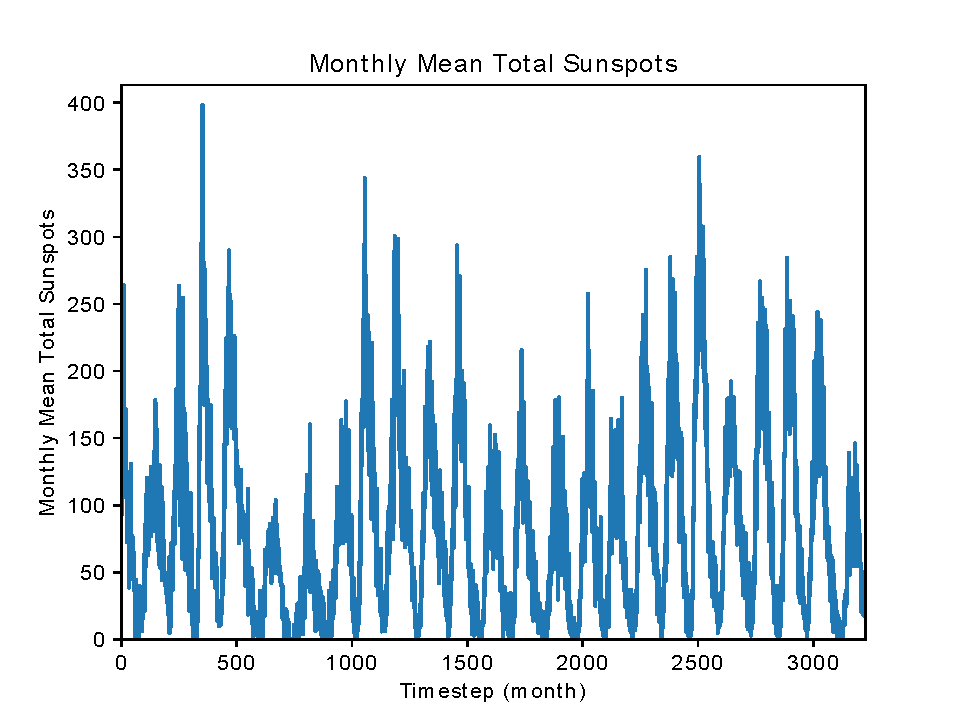
\includegraphics[scale=0.28]{imgs/sunspots.pdf}
  \caption{Monthly mean total sunspots between January 31, 1749 to August 31, 2017 dataset.}\label{fig:sunspots_dataset}
\endminipage\hfill
\minipage{0.32\textwidth}
	\centering
  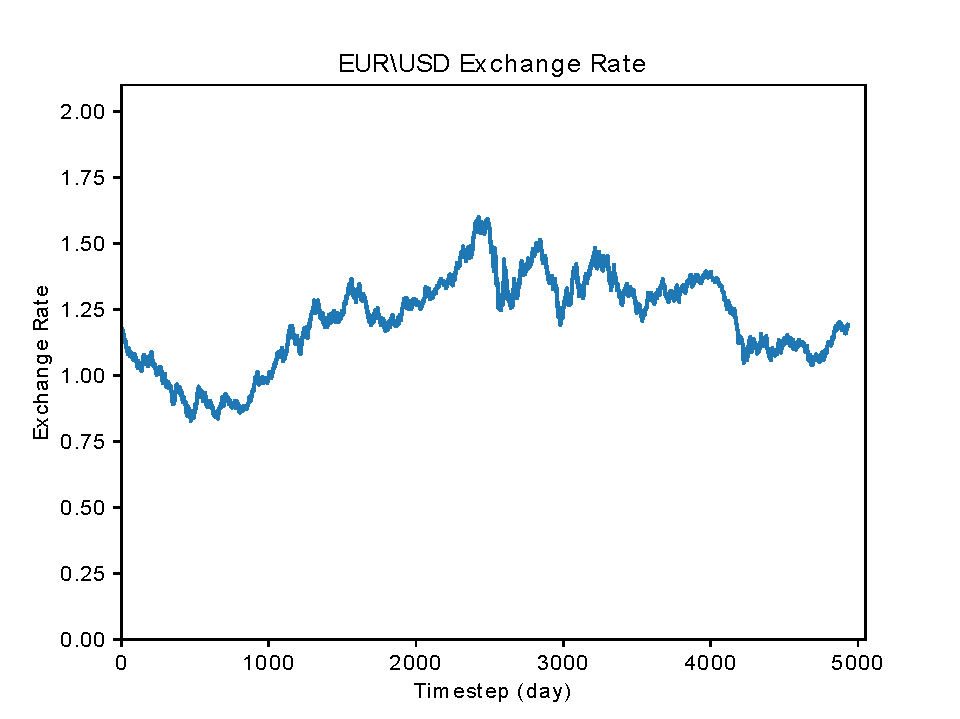
\includegraphics[scale=0.28]{imgs/eurusd.pdf}
  \caption{Daily closing prices of the EUR/USD foreign exchange rate.}\label{fig:eurusd_dataset}
\endminipage\hfill
\minipage{0.32\textwidth}
	\centering
  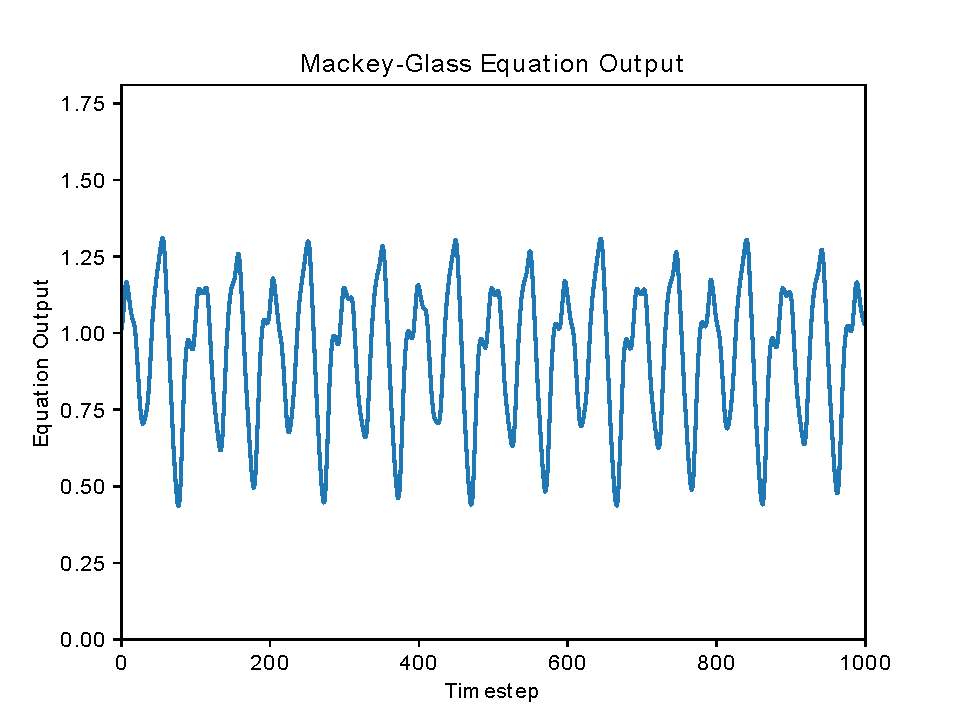
\includegraphics[scale=0.28]{imgs/mackey.pdf}
  \caption{Mackey-Glass nonlinear time delay differential equation output.}\label{fig:mackey_dataset}
\endminipage
\end{figure}

The sunspot dataset is a univariate time series of the monthly average number of sunspots from January 31, 1749 to August 31, 2017 providing 3224 data samples. The dataset is taken from the Solar Influences Data Analysis Center which is the solar physics research department of the Royal Observatory of Belgium \citep{especuloide_2017}. The dataset, shown in \autoref{fig:sunspots_dataset}, shows seasonality with large differences betweens seasons and also exhibits some signs of periodicity approximately every 11 years.

The EUR/USD foreign exchange rate dataset consists of the closing price of the exchange rate's ticker between January 1, 1999 and November 30, 2017 giving 4935 examples for training and testing. Predicting foreign exchange rates is an important task in finance and economics but, due to the complexity of the data, most methods perform poorly on out-of-sample data when compared to a simple random walk model. A plot of this dataset is shown in \autoref{fig:eurusd_dataset}.

The final dataset is the Mackey-Glass time-delay differential equation output introduced by Mackey and Glass \citep{mackey1977oscillation}. The dataset is generated by the Mackey-Glass equation which produces a noisy non-periodic, non-convergent time series that serves as an example of deterministic chaos. This dataset is taken from the \textit{frbs} package in R \citep{frbscitation} which contains 1000 data points and is shown in \autoref{fig:mackey_dataset}. 

To study the ensemble method the dataset is segmented as outlined above after being split into train and test datasets. One-step ahead predictions are made with the trained ensemble and, as data become available, new methods are added to the ensemble. Error measures between predicted and actual values for ADLE, a single LSTM network, and a linear ARIMA model are compared to demonstrate the competitiveness of the model.


\subsection{Results}\label{sec:results}

\begin{table}
	\centering
    \bgroup
	\def\arraystretch{1.5}
	\begin{tabular}{|c|c|c|c|c|c|c|}
		\hline
        & \multicolumn{2}{|c|}{ARIMA} & \multicolumn{2}{|c|}{LSTM} & \multicolumn{2}{|c|}{ADLE}\\ 
        & MAE & MSE & MAE & MSE & MAE & MSE \\
        \hline
        Sunspots & -0.343 & 639.594 & 19.909 & 786.056 & 19.515 & 727.079 \\
        \hline
        EUR/USD Exchange Rate & $2.810e^{-5}$ & $6.470e^{-5}$ & 0.007 & $9.317e^{-5}$ & 0.0097 & $1.690e^{-4}$ \\
        \hline 
        Mackey-Glass Equation & -0.1110 & 0.0634 & 0.0278 & 0.0011 & 0.0274 & 0.00107 \\
        \hline
	\end{tabular}
    \egroup
    \caption{Mean squared error (MSE) and mean average error (MAE) of ARIMA, LSTM, and ADLE over the three datasets.}
    \label{tab:results}
\end{table}

% ARIMA Results -> Mackey-Glass = 0.06347219 mse -0.111048 mae, Sunspots = 639.5936 mse  -0.3427728 mae, EUR/USD  6.470125e-05 mse 2.809628e-05 mae.

% Ensemble Results -> Mackey-Glass = MSE:  0.0010788867240633607 MAE:  0.02744129431952434, Sunspots = MSE:  727.0787723134752 MAE:  19.51531165180737, EURUSD = 0.000169 mse, 0.009701 mae

% Single LSTM Results -> Mackey-Glass = 0.0011034919944924368 mse
% 0.027818130368061064 mae, Sunspots = 786.0563356690645
% 19.90894584367478, EURUSD =  9.316746952916529e-05 mse
% 0.00744148990927441 mae

The datasets described above were split into test and training datasets and used to train an ARIMA model, a single LSTM, and ADLE. To find an acceptable set of hyperparameters for the single LSTM an algorithm similar to population based training, introduced by Jaderberg \citep{DBLP:journals/corr/abs-1711-09846}, was used. To compare performance of the three methods, predictions of the test set are made and mean squared error (MSE) and mean average error (MAE) are computed. These error metrics are defined as 
\begin{align*}
	MAE &= \frac{1}{n} \sum_{i=1}^n |\hat{y_i} - y_i| \\
    MSE &= \frac{1}{n} \sum_{i=1}^n (\hat{y_i} - y_i)^2.
\end{align*}
For this initial implementation of ADLE $k$ in the weighted k-NN aggregation is set as the number of networks in the ensemble. Tuning this hyperparameter may produce better results than those summarized in \autoref{tab:results}.

The results of the ensemble compared to a linear ARIMA model and a single LSTM model are summarized in \autoref{tab:results}. It is shown that in two out of three datasets ADLE performs better than a single LSTM and outperforms both of the other benchmarks on the Mackey-Glass dataset. On the datasets where ADLE underperforms the other methods the results remain competitive and, with more fine tuning, ADLE may have the capability of outperforming the other methods. Due to the nature of discrete time series data, such as the Sunspots and EUR/USD exchange rate datasets, ARIMA models can be expected to fit well for one-step ahead predictions (with retraining at every time step). This is because steps between points is actually a straight line so a good linear measure determining where the line is heading is bound to give good predictions.


%% DIscuss training times as well
\subsubsection{Sunspots} \label{sec:sunspots_results}
\begin{figure}
\centering
\minipage{0.32\textwidth}
	\centering
  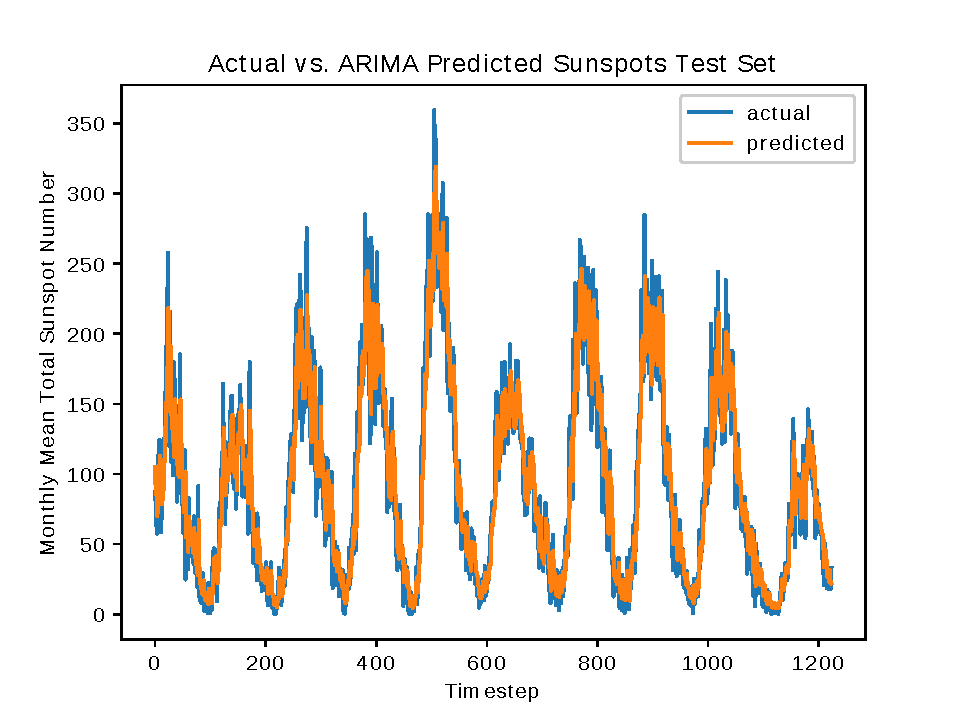
\includegraphics[scale=0.28]{imgs/arima_results_sunspots.pdf}
  \caption{Predicted ARIMA values vs actual values for the sunspots dataset.}\label{fig:sunspots_graph_arima}
\endminipage\hfill
\minipage{0.32\textwidth}
	\centering
  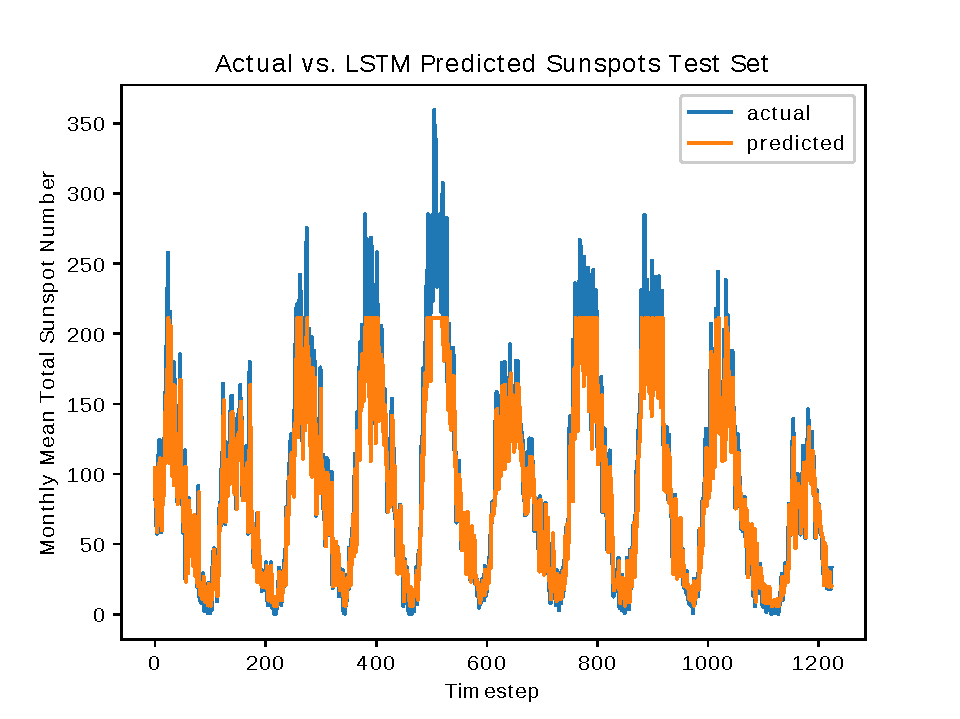
\includegraphics[scale=0.28]{imgs/lstm_results_sunspots.pdf}
  \caption{Predicted LSTM values vs actual values for the sunspots dataset.}\label{fig:sunspots_graph_lstm}
\endminipage\hfill
\minipage{0.32\textwidth}
	\centering
  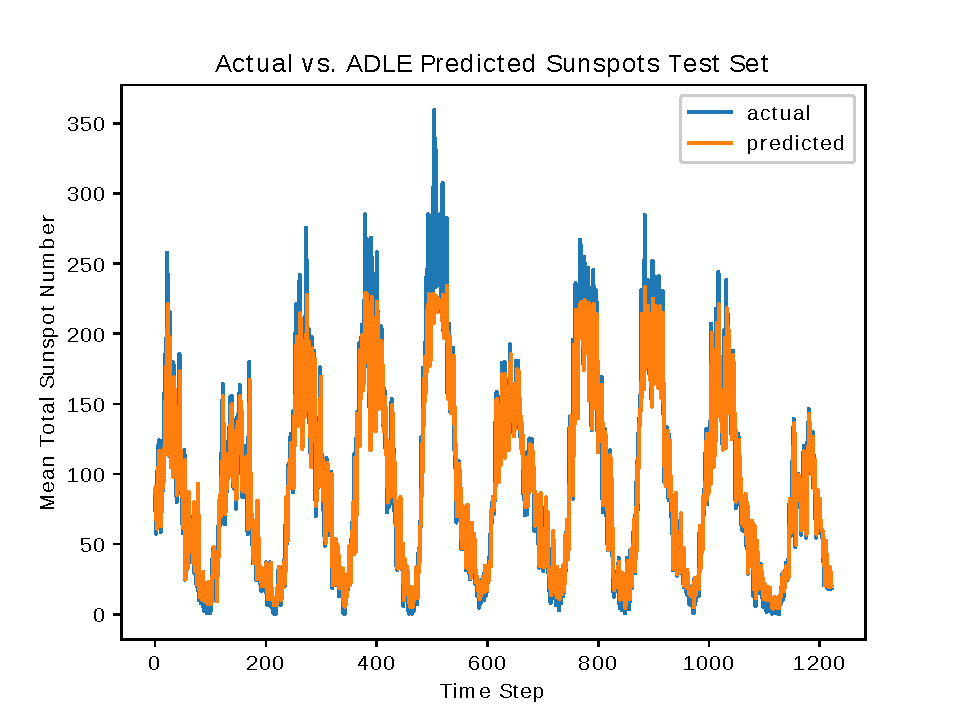
\includegraphics[scale=0.28]{imgs/adle_results_sunspots.pdf}
  \caption{Predicted ADLE values vs actual values for the sunspots dataset.}\label{fig:sunspots_graph_adle}
\endminipage
\end{figure}

Shown in \autoref{fig:sunspots_graph_arima}, \autoref{fig:sunspots_graph_lstm}, and \autoref{fig:sunspots_graph_adle} are the predicted values from ARIMA, LSTM and ADLE vs actual values of the sunspots dataset. It appears that the single LSTM and ADLE do a better job at predicting the mean total sunspots number during periods of `typical' behavior but fail when attempting to predict extraordinarily high values for the number of sunspots. This indicates the models may be restricted in some way when attempting to predict these values which warrants further investigation.

\subsubsection{EUR/USD Exchange Rate}
\begin{figure}
\centering
\minipage{0.32\textwidth}
	\centering
  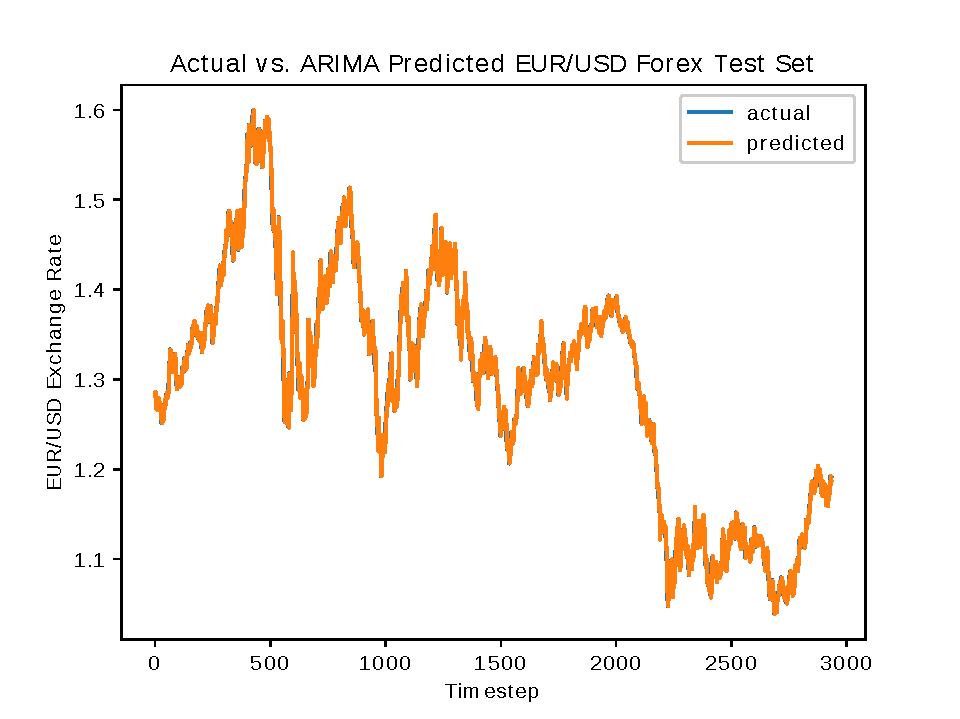
\includegraphics[scale=0.28]{imgs/arima_results_eurusd.pdf}
  \caption{Predicted ARIMA values vs actual values for the EUR/USD exchange rate dataset.}\label{fig:eurusd_graph_arima}
\endminipage\hfill
\minipage{0.32\textwidth}
	\centering
  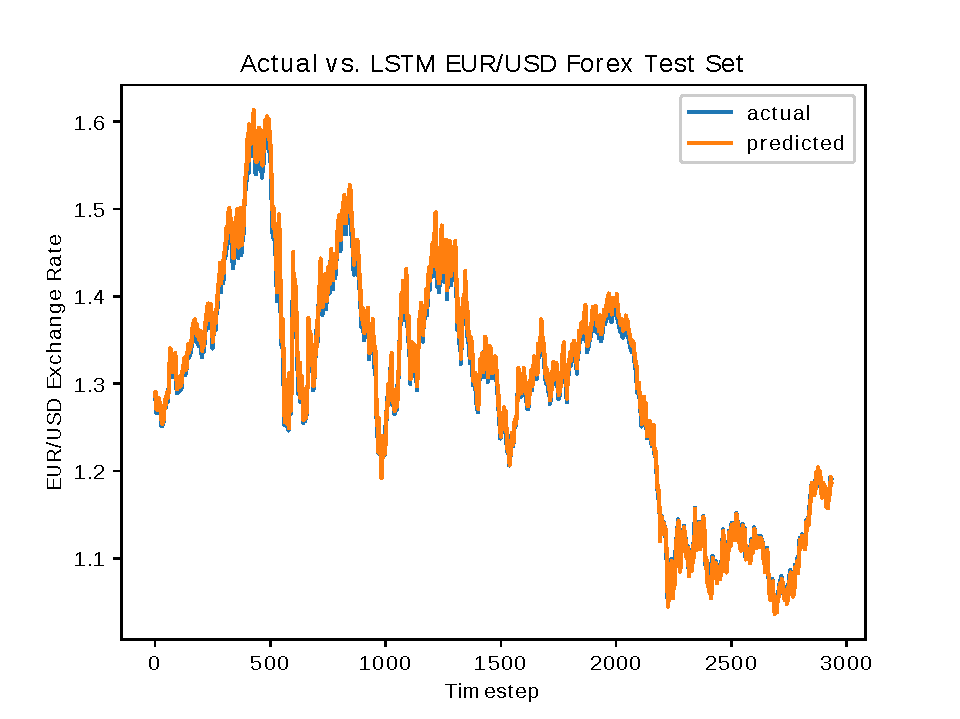
\includegraphics[scale=0.28]{imgs/lstm_results_eurusd.pdf}
  \caption{Predicted LSTM values vs actual values for the EUR/USD exchange rate dataset.}\label{fig:eurusd_graph_lstm}
\endminipage\hfill
\minipage{0.32\textwidth}
	\centering
  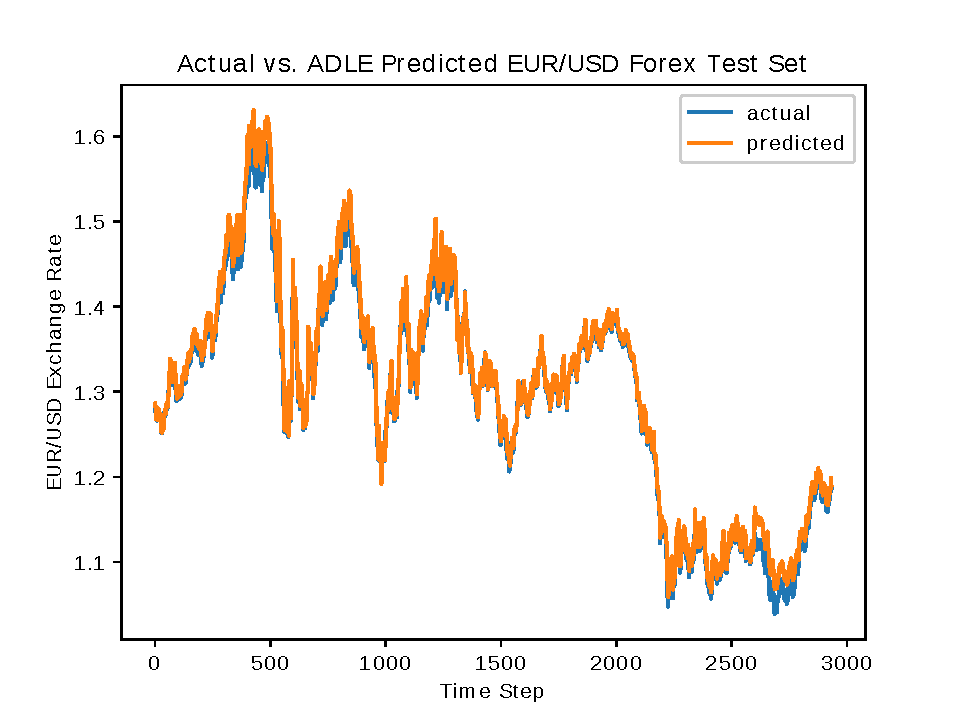
\includegraphics[scale=0.28]{imgs/adle_results_eurusd.pdf}
  \caption{Predicted ADLE values vs actual values for the EUR/USD exchange rate dataset.}\label{fig:eurusd_graph_adle}
\endminipage
\end{figure}

The predicted values compared to actual values of the EUR/USD foreign exchange rate dataset can be seen in \autoref{fig:eurusd_graph_arima}, \autoref{fig:eurusd_graph_lstm}, and \autoref{fig:eurusd_graph_adle} for the ARIMA, LSTM, and ADLE models, respectively. As was seen with the sunspots dataset in \autoref{sec:sunspots_results}, when attempting to predict values that are particularly low or high ADLE has issues meeting these datasets. In both cases for the EUR/USD dataset ADLE's predictions are higher than the expected values indicating too much weight may be placed on the methods predicting high values during these periods (since the initial implementation uses all networks for prediction).


\subsubsection{Mackey-Glass Equation Output}
\begin{figure}
\centering
\minipage{0.32\textwidth}
	\centering
  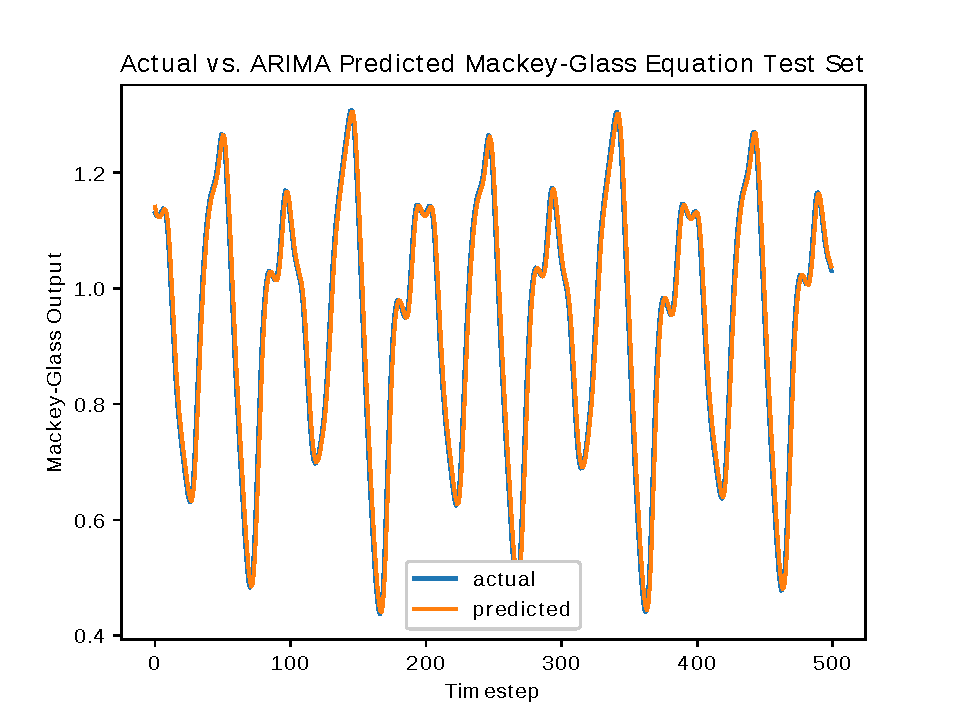
\includegraphics[scale=0.28]{imgs/arima_results_mackey.pdf}
  \caption{Predicted ARIMA values vs actual values for the Mackey-Glass equation output dataset.}\label{fig:mackey_graph_arima}
\endminipage\hfill
\minipage{0.32\textwidth}
	\centering
  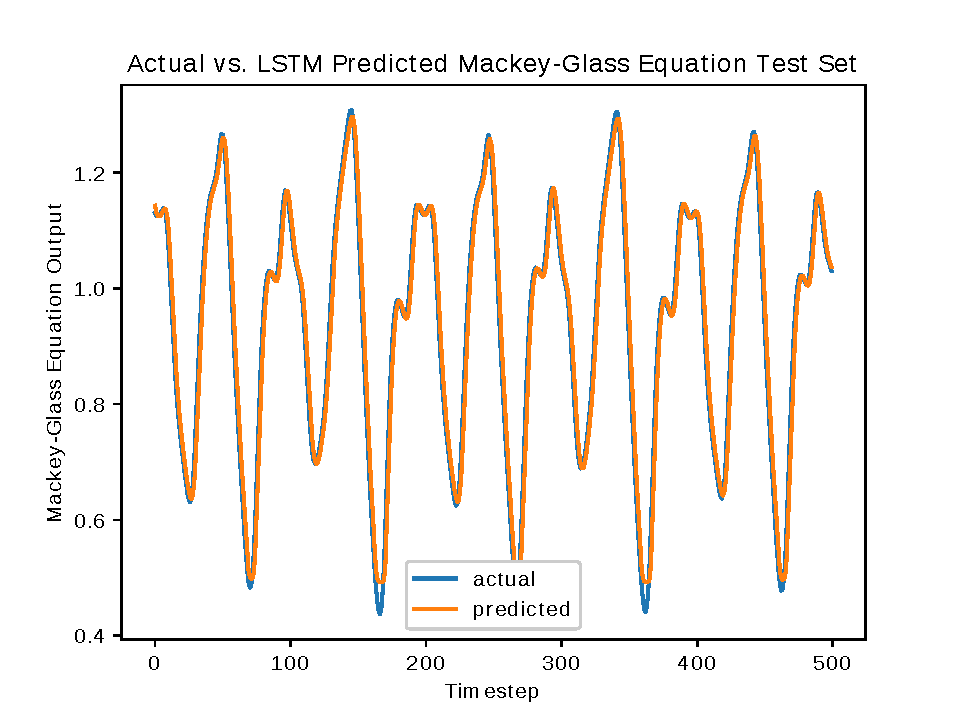
\includegraphics[scale=0.28]{imgs/lstm_results_mackey.pdf}
  \caption{Predicted LSTM values vs actual values for the Mackey-Glass equation output dataset.}\label{fig:mackey_graph_lstm}
\endminipage\hfill
\minipage{0.32\textwidth}
	\centering
  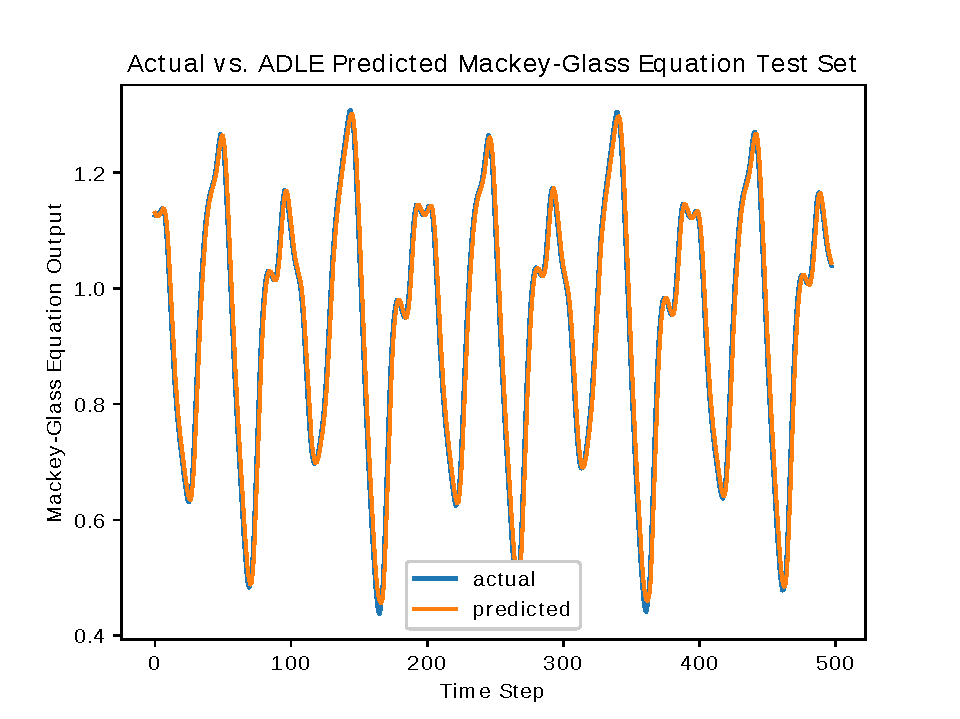
\includegraphics[scale=0.28]{imgs/adle_results_mackey.pdf}
  \caption{Predicted ADLE values vs actual values for the Mackey-Glass equation output dataset.}\label{fig:mackey_graph_adle}
\endminipage
\end{figure}

\autoref{fig:mackey_graph_arima}, \autoref{fig:mackey_graph_lstm}, and \autoref{fig:mackey_graph_adle} show the actual time series values plotted against the ARIMA, LSTM, and ADLE models, respectively. In these figures it's hard to distinguish between the actual and predicted values which indicates the dataset is likely easy to learn. This is expected based on the summarized results in \autoref{tab:results} where it can be seen that all three models have approximately the same performance on this dataset.


\section{Conclusions and Future Work}

\begin{figure}
\centering
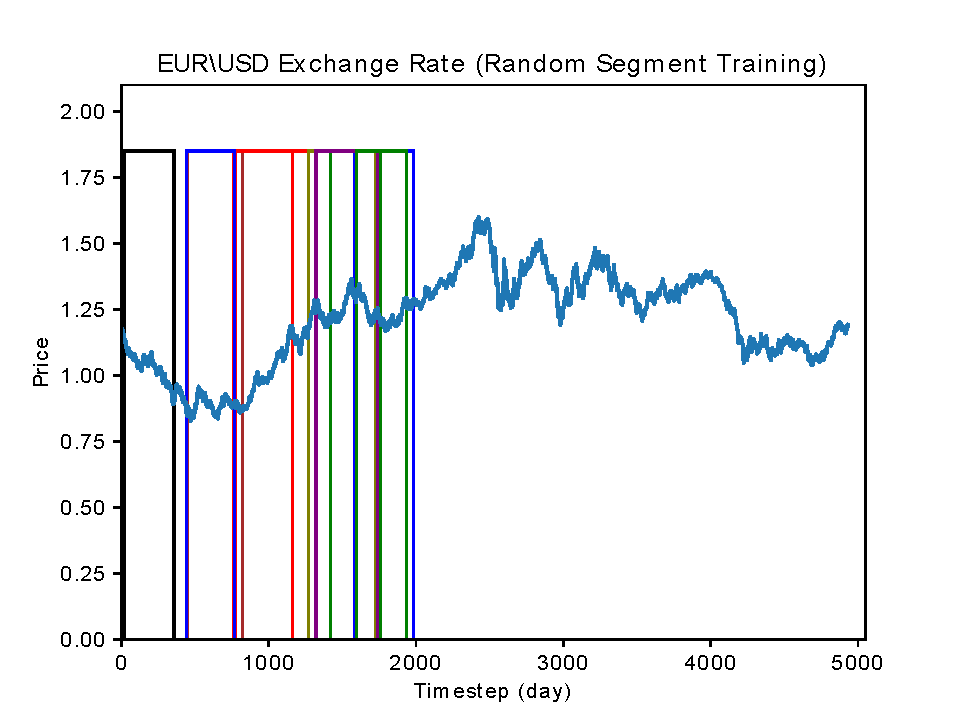
\includegraphics[scale=0.4]{imgs/random_segments_forex.pdf}
   \caption{Training segments when start points and sizes are randomly generated.}\label{fig:random}
\end{figure}

As shown in \autoref{sec:results}, in this limited test ADLE outperforms or performs competitively when compared to standard methods on these datasets. The ensemble works best on the Mackey-Glass and Sunspots datasets which both show signs of periodicity and seasonality indicating that the method may outperform other models on data with similar trends. As with most things, there is no ``one size fits all'' method for time series forecasting but with further refinement it's believed ADLE is a good competitor for a particular type of dataset.  
One thing to note is the results above are preliminary due to the time constraints of the project. Given more time the hyperparameters of each ensemble could be tuned to potentially give better prediction accuracy. 

Some interesting avenues for future work include testing the ensemble on multivariate time series, implementing another training methodology wherein random starting locations and sizes are chosen for each data segment in an attempt to capture the data's structural changes (\autoref{fig:random}), a parallel implementation of the algorithm to decrease training times and improve the efficiency of the method, and the application of different aggregation functions, e.g. a neural network with, online training to weight each individual model's prediction at each time step.

In the current implementation of ADLE the ensemble consists of LSTM-RNNs as the base model. Other promising methods such as convolutional LSTMs, support vector machines, convolutional neural networks and deep belief networks, which have all been shown to be good predictors of time series data, could potentially boost the performance of ADLE. Additional updates to the training procedure could prove beneficial as well. For instance, in the current implementation each LSTM uses the same set of hyperparameters but in reality certain segments of data might be better approximated by networks with fewer or additional hidden layers and training epochs. That is, more linear segments may require shallow, narrow networks while complex segments might need deeper, wider networks to effectively approximate their data generating functions.

Perhaps the most promising future work is to implement a type of change detection to better determine when the underlying structure of the data changes. The goal of ADLE is to find models that best fit the data as statistical properties of the dataset change. This acts as a workaround to the stationarity assumption of machine learning methods. Determining when these changes occur could prove critical to the success of the method. 
  

% Future work, 
% \begin{itemize}
% \item Multivariate time series
% \item Random segment starts and sizes
% \item Many randomly sized segments moving around the training (and new training) data so many segments are covered multiple times but all are covered at least once
% \item Essentially with all of thee above want to be able to find better areas where the statistical properties change or at least make it more probable we land on those boundaries
% \item Parallelization to make training mucho mucho fast
% \item different models to make up ensemble, i.e. lstms, svms, anns, etc.
% \item Adaptive hyperparameters for the models based on complexity of current segment (networks hyperparameters change based on how complex the current segment is, creating better models in all cases rather than attempting to use a generally good model for all plus faster training for simpler portions)
% \item smarter selection of data segments (change detection)
% \item change detection
% \item Data preprocessing \item Data preprocessing 
% \end{itemize}

\bibliography{morast}

\end{document}
